% vim: set textwidth=78 autoindent:

\subsection{Complemento de Texto Delimitado}\label{label_dltext}    

% when the revision of a section has been finalized, 
% comment out the following line:
%\updatedisclaimer

El complemento de texto delimitado permite cargar un archivo de texto delimitado como una capa en QGIS. 

\minisec{Requerimientos}

Para ver un archivo de texto delimitado como una capa, el texto debe contener:

\begin{enumerate}      
\item Una línea de cabecera de nombres de campos. Esta debe ser la primera línea en el archivo de texto.
\item La línea de cabecera debe contener un campo X y Y. Estos campos pueden tener cualquier nombre.
\item Las coordenadas x y y deben ser especificadas como un número. El sistema de coordenadas no es importante.
\end{enumerate}

Como un ejemplo de un archivo de texto válido nosotros importamos el archivo de puntos de datos de elevación 
\filename{elevp.csv} que viene con el conjunto de datos de ejemplo de QGIS (Vea la sección ~\ref{label_sampledata}):

\begin{verbatim} 
X;Y;ELEV
-300120;7689960;13
-654360;7562040;52
1640;7512840;3
[...]
\end{verbatim}

Algunos elementos para notar acerca del archivo de texto son:

\begin{enumerate}
\item El archivo de texto de ejemplo usa \mbox{$;$} como delimitador. Cualquier caracter puede ser usado para delimitar los campos.
\item La primer fila es la fila de cabecera. Contiene los campos X, Y y ELEV.
\item No se usan ({\tt{}"{}}) para delimitar los campos de texto.
\item Las coordenadas x están contenidas en el campo {\em X}.
\item Las coordenadas y están contenidas en el campo {\em Y}.
\end{enumerate}

\minisec{Usando el complemento}
Para usar el complemento primero debe activarlo como se describe en la sección \ref{sec:managing_plugins}.

Haga clic en el nuevo ícono de la barra de herramientas \toolbtntwo{delimited_text}{Añadir Capa de Texto Delimitado} para abrir el diálogo de Texto Delimitado como se muestra en la figura \ref{fig:delim_text_plugin_dialog}.

\begin{figure}[ht]
   \begin{center}
   \caption{Diálogo de Texto Delimitado \nixcaption}\label{fig:delim_text_plugin_dialog}\smallskip
   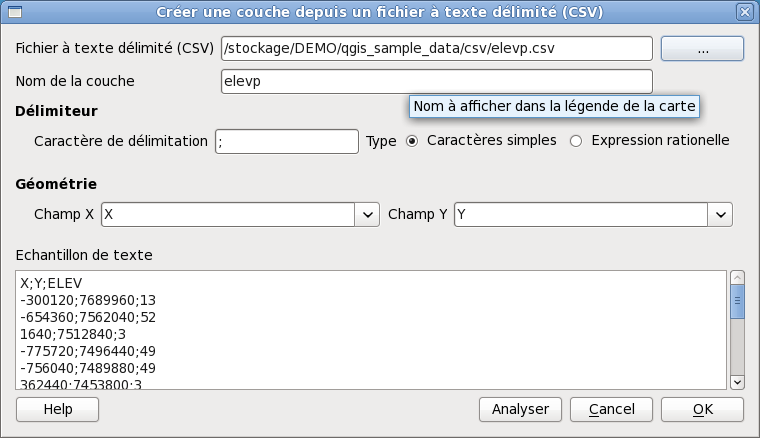
\includegraphics[clip=true, width=9cm]{delimited_text_dialog}
   \end{center}  
\end{figure}

Primero seleccione el archivo (ej., \filename{qgis\_sample\_data/csv/elevp.csv}) para importarlo haciendo clic en el botón \button{Navegar}. Una vez que el archivo es seleccionado, el complemento intenta analizar el archivo usando el último delimitador usado, en este caso un punto y coma (\mbox{$;$}). Para analizar propiamente el archivo, es importante seleccionar el delimitador correcto. Para cambiar el delimitador al tabulador use 
\mbox{$\backslash$}t (esta es una expresión regular para el caracter tabulador).
Despues de cambiar el delimitador, haga clic \button{analizar}.

Una vez que ha analizado el archivo, elija los campos X y Y de la lista desplegable y capture un nombre de capa (ej., \filename{elevp} ) como se muestra en la figura 
\ref{fig:delim_text_plugin_dialog}. Para agregar una capa al mapa, haga clic en
\button{Añadir Capa}. El archivo de texto delimitado ahora se comporta como cualquier otra capa del mapa de QGIS.
